\documentclass[12pt,a4paper]{scrartcl}

%\usepackage{algorithmic}    % Typesetting for pseudocode
%\usepackage{algorithm}      % Formatting for general algorithm blocks
\usepackage{fancyhdr}       % Gives fancy header
\usepackage{mdwlist}        % List related commands
\usepackage{url}            % Nicer URL formatting
\usepackage{new3151defs}    % COMP[39]151 defs

% Automata package
\usepackage{tikz}
\usetikzlibrary{arrows, automata, positioning, shapes}

% Page header
%\pagestyle{fancy}
%\lhead{COMP[39]151 Warmup Assignment
%\rhead{Timothy Wiley, z3109831}

% Line spacing 1.6 for 'double'
%\linespread{2}

% Declare commonly used graphic extensions and precedence
\DeclareGraphicsExtensions{.pdf,.png,.jpg}

\begin{document}

\title{COMP[39]151 Warm-up assignment}
\author{Adi? ?(?) \\ 
        \texttt{?@cse.unsw.edu.au} \\ 
        and \\ 
        Timothy Wiley (z3109831) \\
        \texttt{timothyw@cse.unsw.edu.au} }

\maketitle

%\begin{align}
%  \Not \Always \psi \Eventually y < 5 \Implies v \leq 5
%  &\not\Implies \Next z \Until s \And p \Or \phi\\ 
%  &\Equiv\delta \in \Real\\
%  &\Implies \gamma \geq 10\\
%  & \Exi{x \notin \Integer}{x < \text{Rupert}}
%\end{align}

%\begin{lstlisting}
%\end{lstlisting}

%\begin{figure}[H]
%   \centering
%   \begin{tikzpicture}[->,shorten >=1pt,node distance=3cm,on grid,auto]
%      %\tikzstyle{vertex}=[circle,fill=black!25,minimum size=17pt,inner sep=5pt]
%      %\tikzstyle{state}=[fill=gray,text=black,circle]
%
%      \node[state,initial]    (q0)                    {$q_0$};
%      \node[state]            (in)     [right=of q0]  {booth};
%      \node[state]            (falsum) [above=of in]  {$\bot$};
%      \node[state,accepting]  (dial)   [right=of in]  {dial};
%
%      \path (q0)     edge [loop below]    node {walk}       (q0)
%                     edge                 node {enter}      (in)
%                     edge                 node {dial}       (falsum)
%            (in)     edge                 node {dial}       (dial)
%                     edge [loop below]    node {enter}      (in)
%                     edge                 node {walk}       (falsum)
%            (dial)   edge [loop below]    node {dial,enter} (dial)
%                     edge                 node {walk}       (falsum);
%            %(falsum) edge [loop above]    node {*}          (falsum);
%   \end{tikzpicture}
%   \caption{a (deterministic) FSM for `corridor world'}
%\end{figure}

\section{Question 1}

\subsection{Part A}

Our implementation is:
\lstinputlisting{zeroA.pml}
%\begin{lstlisting}
%\end{lstlisting}

\subsection{Part B}

\subsection{Part C}

\subsection{Part D}

\subsection{Part E}

\section{Question 2}

We defined the Owicki/Gries style proof of the partial correctness of \texttt{zeroE} as
\begin{equation}
    \{ \textrm{$f$ is a function over $\Integer$ with at least one zero} \}
    \texttt{zeroE}
    \{ x \in \Integer \And f(x)=0 \}
\label{eq:og-proof}
\end{equation}

For the proof, we constructed the transition diagram for process $P$ (Figure \ref{fig:p-trans}) and the transition diagram for $Q$ (Figure \ref{fig:q-trans}).
Each state corresponds to the appropriate line of code in the processes and assertions at each state are given in blue.

To aid in the proof we defined two global auxiliary boolean variables $fP$ and $fQ$.
These variables are true if states $p6$ and $q6$ have ever been visited respectively, and are false otherwise.
To achieve this, both variables are initially set to false, and are set to true when transitioning into their respective states $p6$ or $q6$.

We then introduce the global invariant
\begin{equation}
    I: \quad found = fP \Or fQ
\label{eq:og-invariant}
\end{equation}
This invariant is maintained at every state as:
\begin{enumerate}
    \item Initially all three variables $found$, $fP$ and $fQ$ are false.
    \item In the states that change $found$, $fP$ or $fQ$.
    \begin{enumerate}
        \item State $p6$ sets both $found$ and $fP$ to true, maintaining the invariant.
        \item Likewise, state $q6$ sets both $found$ and $fQ$ to true, maintaining the invariant.
    \end{enumerate}
\end{enumerate}

The assertions on the transition diagrams can now be established. Consider the transition diagram for $P$. The assertions are proven as follows:
\begin{enumerate}
    \item At all states: $\{i\ge0\}$ is true as initially $i:=0$ and the only transition to alter $i$ is $p3 -> p4$ which increments $i$.
    \item At $p2$: $\{!fP\}$ is derived from the transition condition and $I$. There is no interference as $Q$ does not alter $fP$.
    \item At $p3$ and $p4$: $\{!fP\}$ is maintained as $fP$ is not altered. There is no interference as $Q$ does not alter $fP$.
    \item At $p5$: $\{f(i)=0\}$ is given from the transition condition and there is no interference as $i$ is local to $P$.
    \item At $p6$: $\{f(i)=0\}$ is given as $i$ is unchanged. $\{fP\}$ is given from the transition action. There is no interference as $Q$ does not alter $i$ or $fP$.
    \item At $p1$: $\{fP \rightarrow f(i)=0\}$ named $a1$, is given by the transitions into $p1$ from $p4$ and $p6$.
          From $p4$, the assertion $\{!fP\}$ makes $a1$ trivially true.
          From $p6$ the assertions $\{fP\}$ and $\{f(i)=0\}$ ensure $a1$ is true.
    \item At $p7$: the assertion $\{fP \rightarrow f(i)=0\}$ is maintained as either $fP$ or $i$ is changed, and there is no interference as neither is modified by $Q$.
\end{enumerate}

The assertions on the transition diagram for $Q$ can be established in a similar way, so we do not detail them here.

We finally must establish the assertions at the terminal states of $P$ and $Q$ imply the overall partial correctness for \texttt{zeroE}.
The set of assertions from the terminal states $p7$ and $q7$ are:
\begin{align*}
    I: \quad found &= fP \Or fQ \\
    fo&und \\
    i &\ge 0 \\
    j &\le 1 \\
    fP &\rightarrow f(i) = 0 \\
    fQ &\rightarrow f(j) = 0
\end{align*}

Given $found$ and $I$, the implications can be collapsed to give
\begin{align*}
    i &\ge 0 \\
    j &\le 1 \\
    f(i) = 0 &\Or f(j) = 0
\end{align*}

Finally, as the combined values of $i$ and $j$ cover $\Integer$, we can conclude what was required, that is
\begin{equation}
    x \in \Integer \And f(x) = 0
\label{eq:og-conclusion}
\end{equation}

\begin{figure}[H]
   \centering
   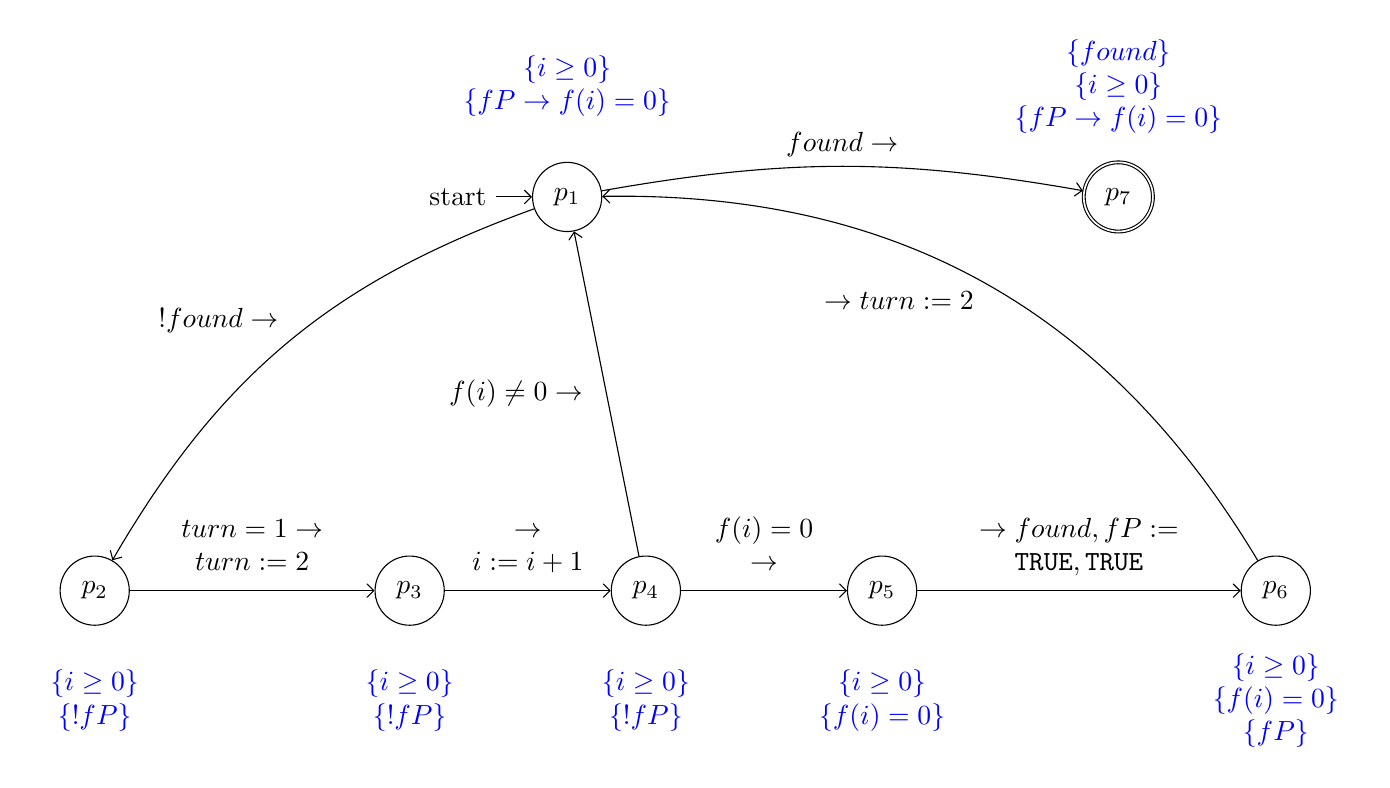
\begin{tikzpicture}[->,>=angle 90,node distance=1.4cm, on grid,auto]

   % Nodes
      \node[state,initial]    (p1)  at (6,5)    {$p_1$};
      \node[state,accepting]  (p7)  at (13,5)   {$p_7$};
      \node[state]            (p2)  at (0,0)    {$p_2$};
      \node[state]            (p3)  at (4,0)    {$p_3$};
      \node[state]            (p4)  at (7,0)    {$p_4$};
      \node[state]            (p5)  at (10,0)   {$p_5$};
      \node[state]            (p6)  at (15,0)   {$p_6$};

   % O/G Assertions
      \node [blue] [above=of p1]  {$\begin{array}{c} \{i \ge 0\} \\ \{fP \rightarrow f(i) = 0\} \end{array}$};
      \node [blue] [above=of p7]  {$\begin{array}{c} \{found\} \\ \{i \ge 0\} \\ \{fP \rightarrow f(i) = 0\} \end{array}$};
      \node [blue] [below=of p2]  {$\begin{array}{c} \{i \ge 0\} \\ \{!fP\} \end{array}$};
      \node [blue] [below=of p3]  {$\begin{array}{c} \{i \ge 0\} \\ \{!fP\} \end{array}$};
      \node [blue] [below=of p4]  {$\begin{array}{c} \{i \ge 0\} \\ \{!fP\} \end{array}$};
      \node [blue] [below=of p5] {$\begin{array}{c} \{i \ge 0\} \\ \{f(i) = 0\} \end{array}$};
      \node [blue] [below=of p6] {$\begin{array}{c} \{i \ge 0\} \\  \{f(i) = 0 \} \\ \{fP\}\end{array}$};

   % Paths
      \path (p1) edge [bend right=20] node[above left] {$!found \rightarrow$} (p2)
                 edge [bend left=10] node[above] {$found \rightarrow$} (p7);
      \path (p2) edge [bend right=00] node[above] {$\begin{array}{c} turn=1 \rightarrow \\ turn:=2 \end{array}$} (p3);
      \path (p3) edge [bend right=00] node[above] {$\begin{array}{c} \rightarrow \\ i:=i+1\end{array}$} (p4);
      \path (p4) edge [bend right=00] node[left]  {$\begin{array}{c} f(i) \ne 0 \rightarrow \end{array}$} (p1)
                 edge [bend right=00] node[above] {$\begin{array}{c} f(i) = 0 \\ \rightarrow \end{array}$} (p5);
      \path (p5) edge [bend right=00] node[above] {$\begin{array}{c} \rightarrow found,fP := \\ \texttt{TRUE},\texttt{TRUE} \end{array}$} (p6);
      \path (p6) edge [bend right=30] node[auto]  {$\rightarrow turn := 2$} (p1);
   \end{tikzpicture}
   \caption{Transition Diagram for process P with assertions in blue}
   \label{fig:p-trans}
\end{figure}

\begin{figure}[H]
   \centering
   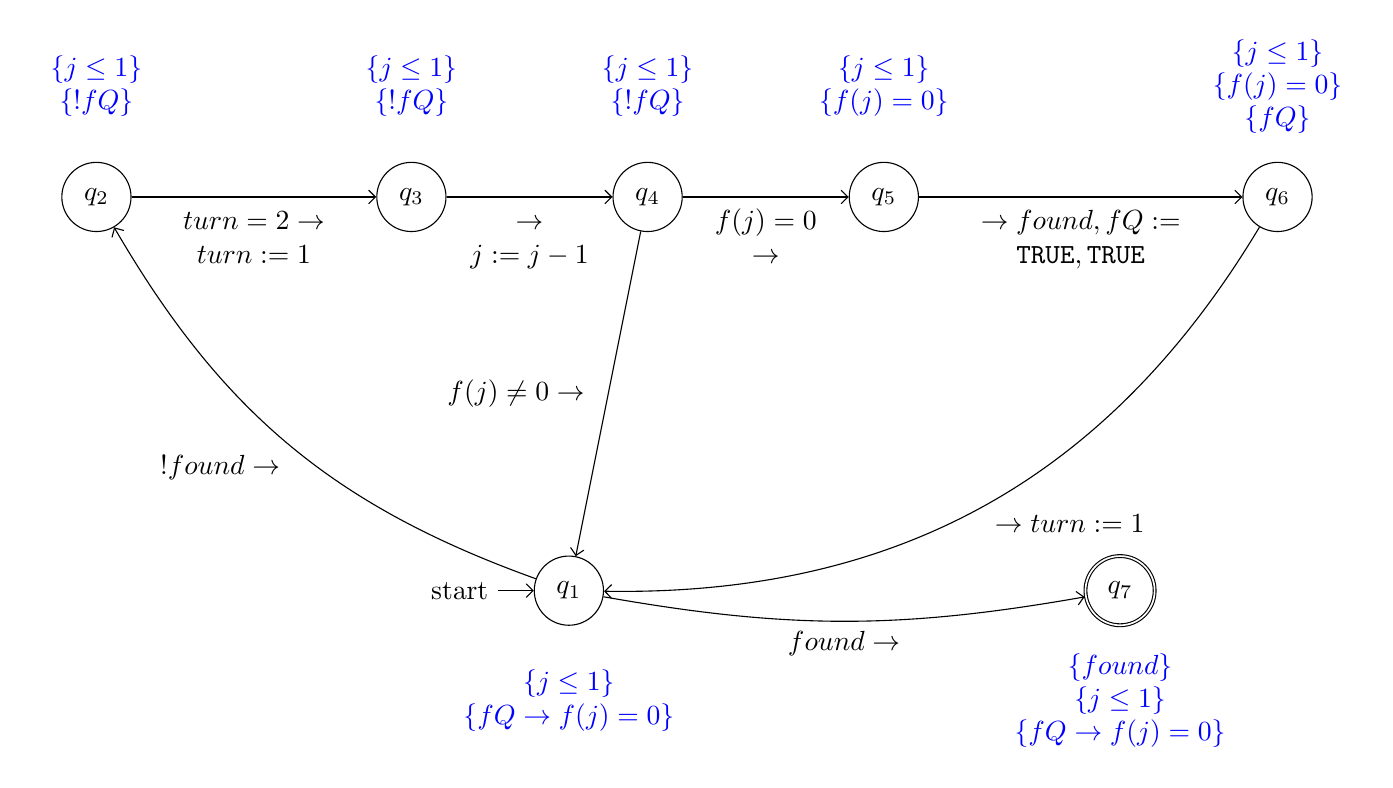
\begin{tikzpicture}[->,>=angle 90,node distance=1.4cm, on grid,auto]

   % Nodes
      \node[state,initial]    (q1)  at (6,-5)    {$q_1$};
      \node[state,accepting]  (q7)  at (13,-5)   {$q_7$};
      \node[state]            (q2)  at (0,0)    {$q_2$};
      \node[state]            (q3)  at (4,0)    {$q_3$};
      \node[state]            (q4)  at (7,0)    {$q_4$};
      \node[state]            (q5)  at (10,0)   {$q_5$};
      \node[state]            (q6)  at (15,0)   {$q_6$};

   % O/G Assertions
      \node [blue] [below=of q1]  {$\begin{array}{c} \{j \le 1\} \\ \{fQ \rightarrow f(j) = 0\} \end{array}$};
      \node [blue] [below=of q7]  {$\begin{array}{c} \{found\} \\ \{j \le 1\} \\ \{fQ \rightarrow f(j) = 0\} \end{array}$};
      \node [blue] [above=of q2]  {$\begin{array}{c} \{j \le 1\} \\ \{!fQ\} \end{array}$};
      \node [blue] [above=of q3]  {$\begin{array}{c} \{j \le 1\} \\ \{!fQ\} \end{array}$};
      \node [blue] [above=of q4]  {$\begin{array}{c} \{j \le 1\} \\ \{!fQ\} \end{array}$};
      \node [blue] [above=of q5] {$\begin{array}{c} \{j \le 1\} \\ \{f(j) = 0\} \end{array}$};
      \node [blue] [above=of q6] {$\begin{array}{c} \{j \le 1\} \\  \{f(j) = 0 \} \\ \{fQ\}\end{array}$};

   % Paths
      \path (q1) edge [bend left=20] node[below left] {$!found \rightarrow$} (q2)
                 edge [bend right=10] node[below] {$found \rightarrow$} (q7);
      \path (q2) edge [bend left=00] node[below] {$\begin{array}{c} turn=2 \rightarrow \\ turn:=1 \end{array}$} (q3);
      \path (q3) edge [bend left=00] node[below] {$\begin{array}{c} \rightarrow \\ j:=j-1\end{array}$} (q4);
      \path (q4) edge [bend left=00] node[left]  {$\begin{array}{c} f(j) \ne 0 \rightarrow \end{array}$} (q1)
                 edge [bend left=00] node[below] {$\begin{array}{c} f(j) = 0 \\ \rightarrow \end{array}$} (q5);
      \path (q5) edge [bend left=00] node[below] {$\begin{array}{c} \rightarrow found,fQ := \\ \texttt{TRUE},\texttt{TRUE} \end{array}$} (q6);
      \path (q6) edge [bend left=30] node[auto]  {$\rightarrow turn := 1$} (q1);
   \end{tikzpicture}
   \caption{Transition Diagram for process Q with assertions in blue}
   \label{fig:q-trans}
\end{figure}

\end{document}
